\documentclass[11pt]{article}\usepackage{knitr}

%AMS-TeX packages
\usepackage{amssymb,amsmath,amsthm} 
%geometry (sets margin) and other useful packages
\usepackage[margin=1in]{geometry}
\usepackage{graphicx, ctable, booktabs}
\usepackage{color}
\usepackage{listings}
\usepackage{ltablex, calc, enumerate, multirow, float, soul, paralist}
\usepackage{hyperref}
\usepackage{longtable, pdflscape, textcase}
\usepackage[backend=bibtex, natbib=true]{biblatex}
\addbibresource{references/refs.bib}
\IfFileExists{upquote.sty}{\usepackage{upquote}}{}

\begin{document}









\setlength{\parskip}{3ex}
\setlength{\parindent}{0pt}

\title{Putting Down Roots: A Graphical Exploration of Community Attachment}
\author{Andee Kaplan, Eric Hare}

\maketitle

\setcounter{page}{1}
\section*{Introduction}

This is the introduction.

\subsection*{Philosophy}
The goal of our work is to facilitate understanding of why people feel attachment to their communities through the use of an interactive and web-based approach. Specifically, we took the point of view of a community planner, either from one of the communities in the study or from a community in the same region or a similar urbanicity. By putting the user in the driver seat of their own experience, we allow the user to apply the conclusions of their interaction to their own situation.


\section*{Technology}

In order to explore the dataset we first created an interactive tool to facilitate the emergence of interesting or descriptive patterns. The construction and design of this tool are detailed in the following sections.

\subsection*{Description and Design}
The interactive tool is comprised of three pieces, \begin{inparaenum}[\itshape 1\upshape)]
\item Control panel, 
\item Map Panel, and
\item Plot panel.
\end{inparaenum}
As the user interacts with each piece, the remaining portions of the interface update to reflect the interaction. In this way we have built an interactive graphic, rather than an animation.

\begin{figure}[H]
\centering
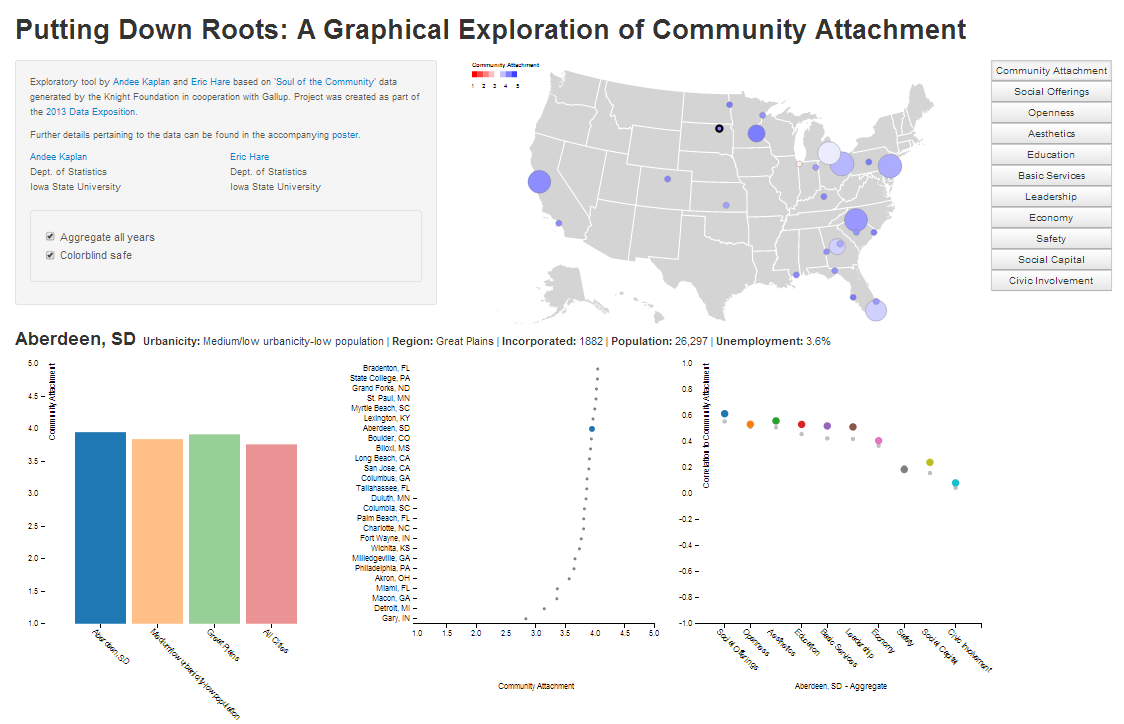
\includegraphics[width=\textwidth]{images/tool.png}
\caption{\label{fig:tool} The components that make up the interactive web interface, (1) Control panel, (2) Map panel, and (3) Plot panel.}
\end{figure}



\subsection*{The Shoulders of Giants}

\subsection*{Why?}
During the creation of our interactive tool, we found it useful to stop and ask, ``Why?'' This process enabled the type of introspection necessary to help ensure usability and relevance in a project of this type.

\subsubsection*{Interactive}
Why interactive? In order to discover what the data has to tell the world. In the words of John Tukey, "Exploratory data analysis is detective work - numerical detective work - or counting detective work - or \emph{graphical detective work}." \cite{tukey77} Dynamic, interactive visualizations can empower people to explore the data for themselves as well as encourage engagement with the data in a way that static visualizations cannot.

\subsubsection*{Linked Plots}
Why linked plots? Linking multiple visualizations shows different aspects of a complex data set and helps highlight relationships. By allowing actions in one plot to affect elements in other plots, comparisons are made easy for the user without requiring much memorization. This aids in pattern finding by avoiding taxation of the user's brain through memorization.

\subsubsection*{Web-based}
Why web-based? A web-based application is platform-independent and allows the user to employ the tool without any software to download. Additionally, by building an application that works on all modern browsers and operating systems, there are no limitations on who can use the tool. Finally, automatic feature additions and bug fixes can be completed transparently to the user.


\section*{Stories}

We elected to divide our analysis using two primary factors. The first is the geographic region the community is located in, and the second is the urbanicity of the particular community. Urbanicity is a census designation which was provided in the dataset, while regions were determined by us. The regions are a rough guideline and do not correspond to any commonly used or accepted regional boundaries. They were merely a method we used to cluster communities into more-alike regions in terms of geography and culture. The interactive tool was then used to help us discover a story in the data for each of the five regions. A map of the regions is displayed in Figure \ref{fig:region_map}.

\begin{knitrout}
\definecolor{shadecolor}{rgb}{0.969, 0.969, 0.969}\color{fgcolor}\begin{figure}[H]

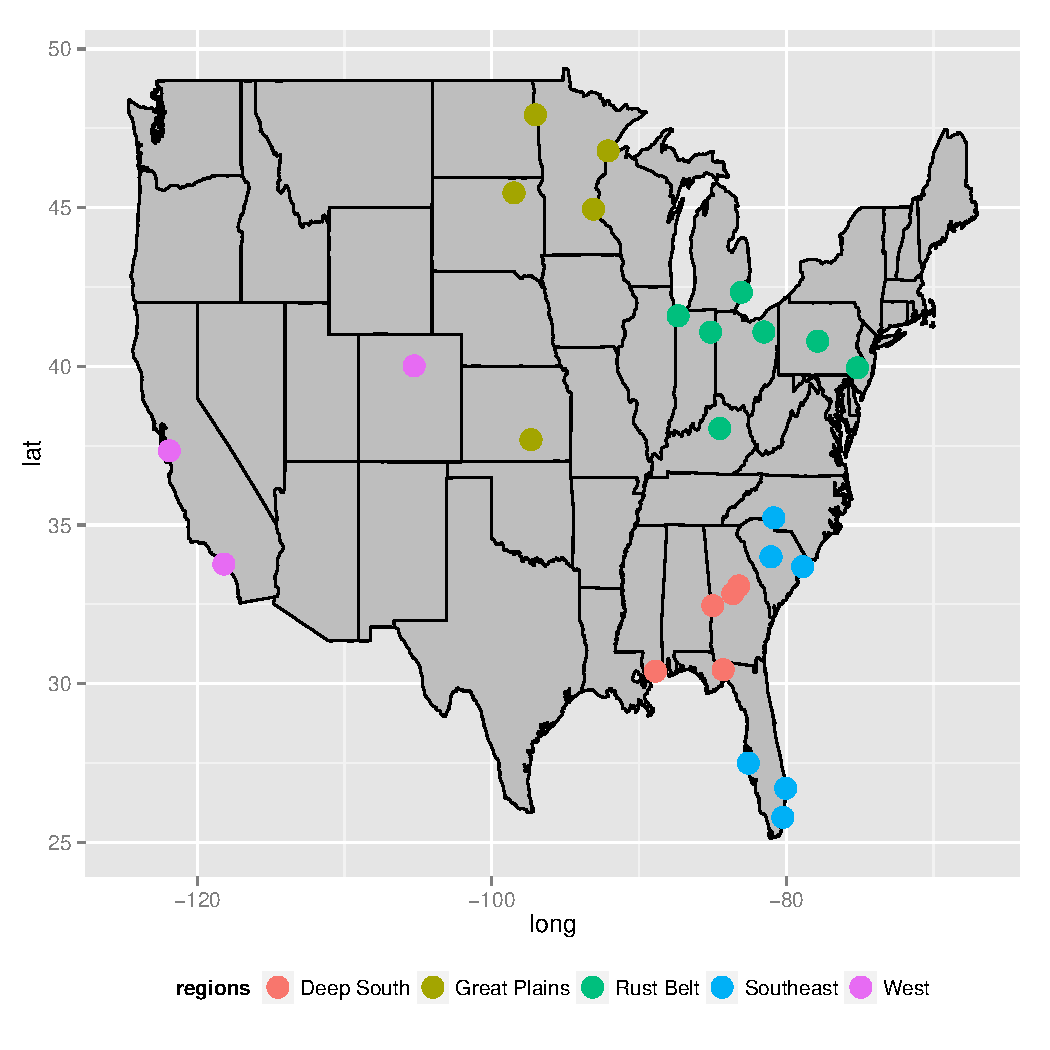
\includegraphics[width=\maxwidth]{figure/region_map} \caption[Map of the five regions to which we assigned the communities]{Map of the five regions to which we assigned the communities.\label{fig:region_map}}
\end{figure}


\end{knitrout}


\subsection*{Great Plains}
The five communities comprosing the Great Plains are Grand Forks, ND, Duluth, MN, Aberdeen, SD, Saint Paul, MN, and Wichita, KS. Through use of the interactive tool, we quickly discovered that the individuals in this region tended to rate the quality of education in the community more highly. In Table \ref{tbl:edu_table}, the top eight communities by the Education Metric are displayed. It can be seen that the Great Plains region includes three of the top four, and four of the top eight communities in terms of Education. Grand Forks, ND in particular has the highest average response for this metric amongst all communities. This is perhaps not too surprising given the presence of the University of North Dakota in this community.

% latex table generated in R 3.0.2 by xtable 1.7-1 package
% Wed Jan  1 08:08:34 2014
\begin{table}[ht]
\centering
\begin{tabular}{lll}
  \hline
Region & Community & Education \\ 
  \hline
Great Plains & Grand Forks, ND & 2.40008396305626 \\ 
  Rust Belt & State College, PA & 2.36484245439469 \\ 
  Great Plains & Aberdeen, SD & 2.25540765391015 \\ 
  Great Plains & St. Paul, MN & 2.13178082191781 \\ 
  West & Boulder, CO & 2.12939698492462 \\ 
  Rust Belt & Philadelphia, PA & 2.10063523905048 \\ 
  Deep South & Tallahassee, FL & 2.09482038429407 \\ 
  Great Plains & Duluth, MN & 2.09265442404007 \\ 
   \hline
\end{tabular}
\caption{Top Six Communities by the Education Metric.} 
\label{tbl:edu_table}
\end{table}



We can visualize the distribution of the Education metric values for each of the Great Plains communities compared to all other communities. Histograms of these values are displayed in Figure \ref{fig:gp_one}. With the exception of Wichita, KS, the Great Plains communities have more responses in the higher values when compared with communities in other regions. This is most visible in both Grand Forks, ND and Aberdeen, SD.

\begin{knitrout}
\definecolor{shadecolor}{rgb}{0.969, 0.969, 0.969}\color{fgcolor}\begin{figure}[H]

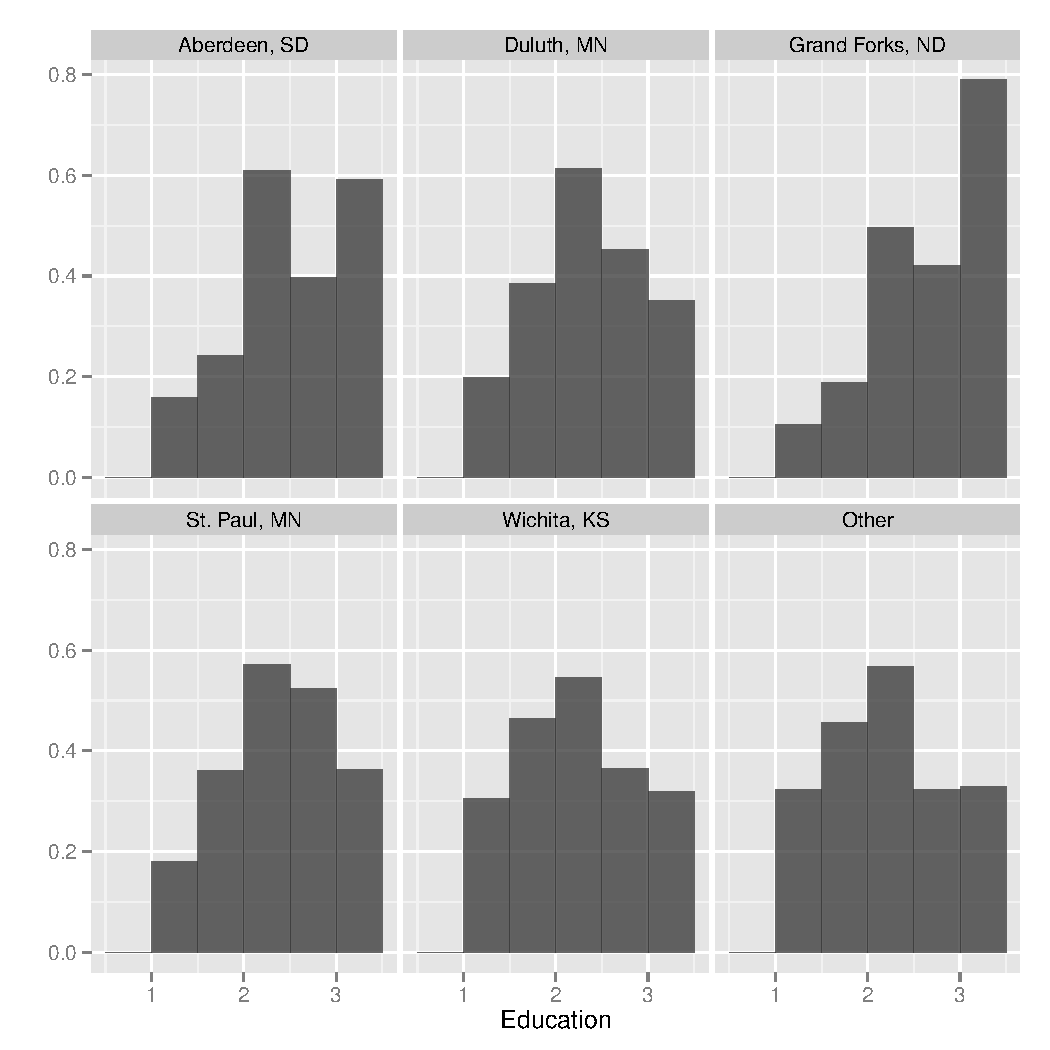
\includegraphics[width=\maxwidth]{figure/gp_one} \caption[Caption]{Caption...\label{fig:gp_one}}
\end{figure}


\end{knitrout}


What might be more surprising is illustrated in Table \ref{tbl:cce_table}; the Great Plains region itself has the largest overall Community Attachment among the five regions. As it turns out, the correlation of the Education metric to the Community Attachment metric in the Great Plains is 0.49. This compares to a correlation of 0.46 in the communities outside the Great Plains. This correlation is illustrated in Figure \ref{fig:gp_two}. The mean response for Community Attachment is plotted versus the mean response for Education in each of the Great Plains communities, and all other communities aggregated. The big dots represent the data aggregated over all years, while the smaller dots represent 2008, 2009, and 2010. A pretty strong relationship between Education and Community Attachment can be observed, but with one notable exception: Saint Paul, MN. Saint Paul has a much higher Community Attachment given its value for Education than what would be expected by observing the other communities. This is likely due Saint Paul's size and cultural presence, which may contribute to other factors which lead to a high sense of Community Attachment.

% latex table generated in R 3.0.2 by xtable 1.7-1 package
% Wed Jan  1 08:08:40 2014
\begin{table}[ht]
\centering
\begin{tabular}{lr}
  \hline
Region & Community Attachment \\ 
  \hline
Deep South & 3.736 \\ 
  Great Plains & 3.916 \\ 
  Rust Belt & 3.568 \\ 
  Southeast & 3.809 \\ 
  West & 3.915 \\ 
   \hline
\end{tabular}
\caption{The average value for the Community Attachment metric in each of the five regions.} 
\label{tbl:cce_table}
\end{table}



\begin{knitrout}
\definecolor{shadecolor}{rgb}{0.969, 0.969, 0.969}\color{fgcolor}\begin{figure}[H]

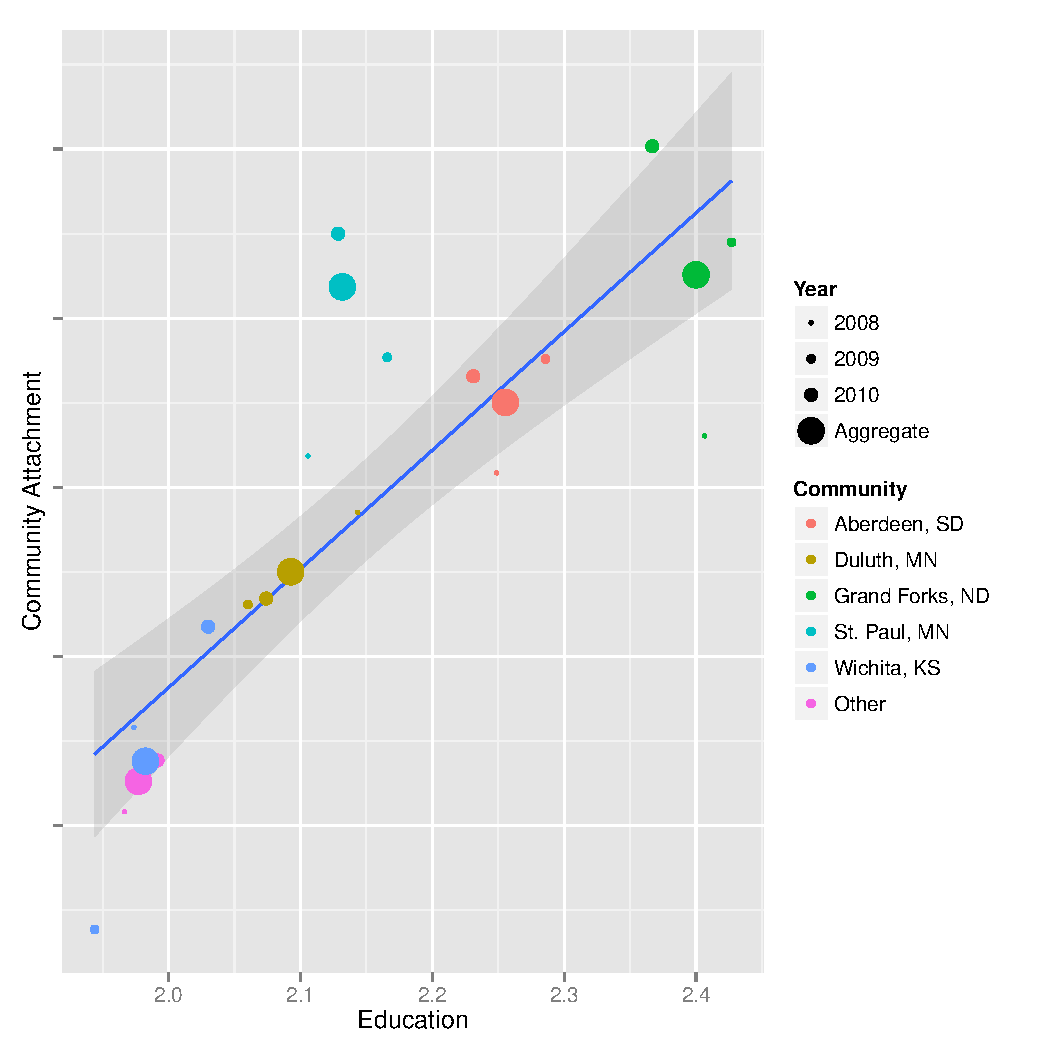
\includegraphics[width=\maxwidth]{figure/gp_two} \caption[Mean Community Attachment value versus mean Education value]{Mean Community Attachment value versus mean Education value. The size of the dots represent the year, while the color represents the community.\label{fig:gp_two}}
\end{figure}


\end{knitrout}



\subsection*{West}
\begin{knitrout}
\definecolor{shadecolor}{rgb}{0.969, 0.969, 0.969}\color{fgcolor}\begin{figure}[H]

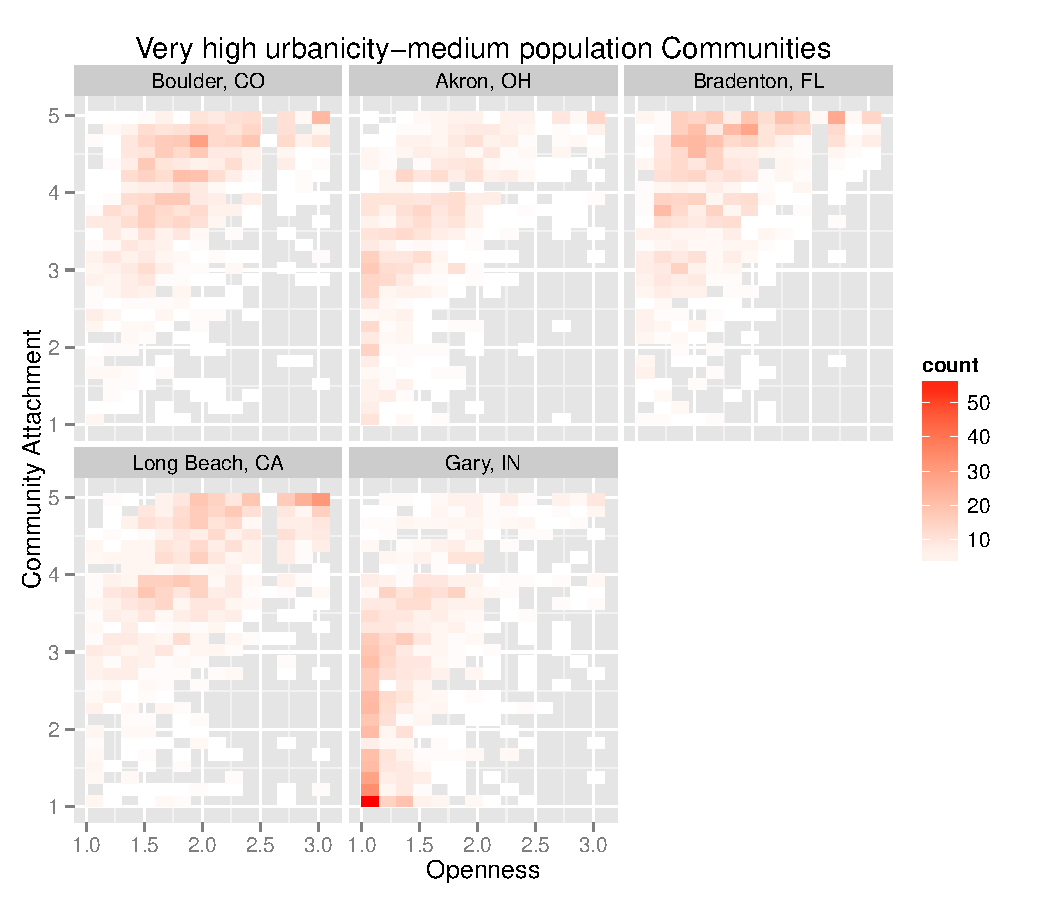
\includegraphics[width=\maxwidth]{figure/west_one} \caption[Caption]{Caption...\label{fig:west_one}}
\end{figure}


\end{knitrout}



\subsection*{Deep South}
\begin{knitrout}
\definecolor{shadecolor}{rgb}{0.969, 0.969, 0.969}\color{fgcolor}\begin{figure}[H]

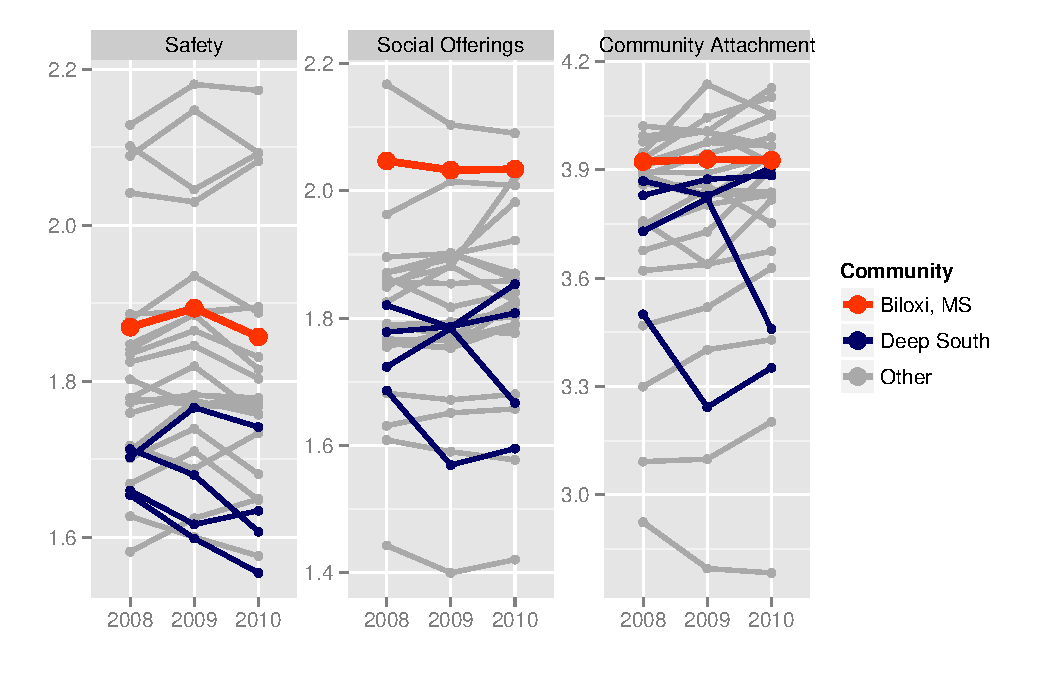
\includegraphics[width=\maxwidth]{figure/ds_one} \caption[Caption]{Caption...\label{fig:ds_one}}
\end{figure}


\end{knitrout}


\subsection*{Southeast}
\begin{knitrout}
\definecolor{shadecolor}{rgb}{0.969, 0.969, 0.969}\color{fgcolor}\begin{figure}[H]

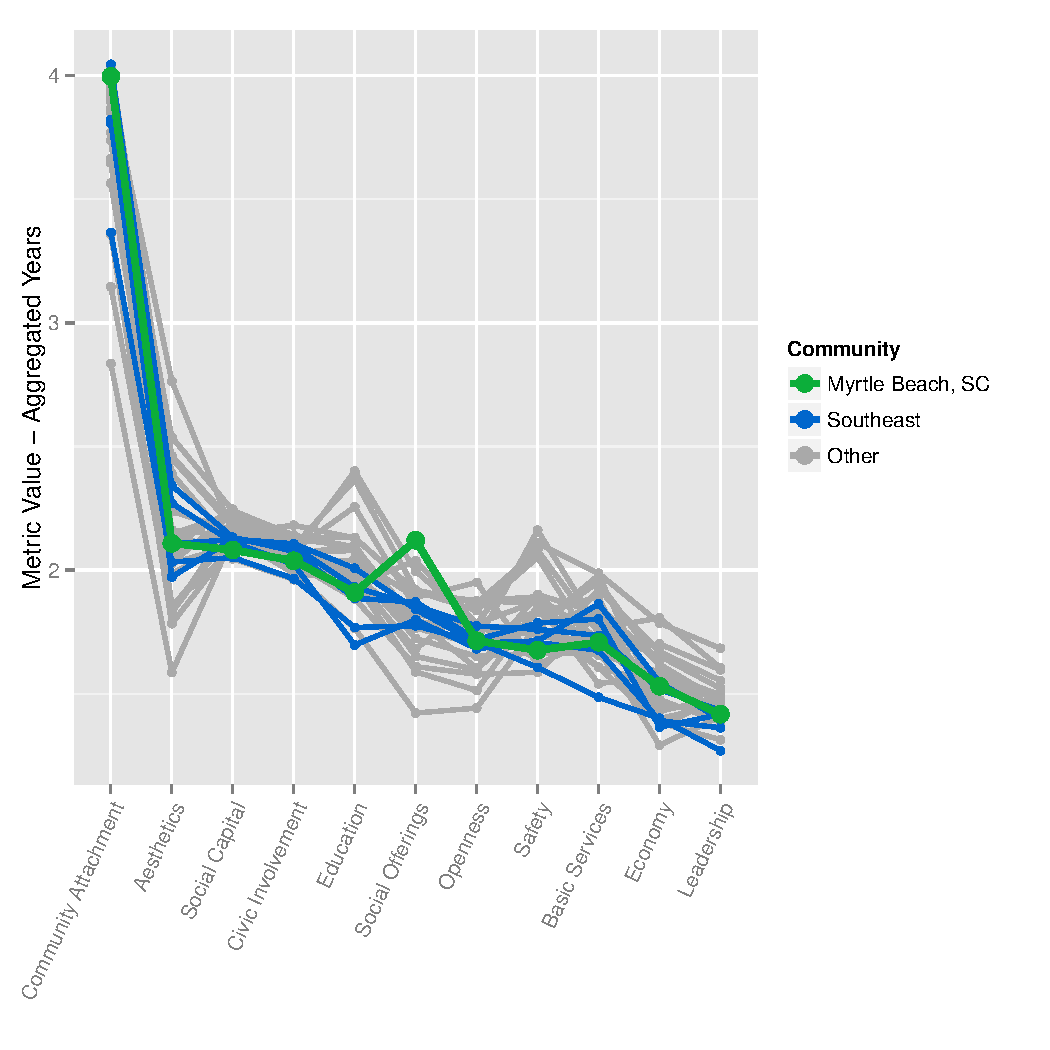
\includegraphics[width=\maxwidth]{figure/southeast_one} \caption[Mean value of metric for each community]{Mean value of metric for each community. Myrtle Beach is highlighted in green, and the other communities in the Southeast are highlighted in blue.\label{fig:southeast_one}}
\end{figure}


\end{knitrout}


\subsection*{Rust Belt}
\begin{knitrout}
\definecolor{shadecolor}{rgb}{0.969, 0.969, 0.969}\color{fgcolor}\begin{figure}[H]

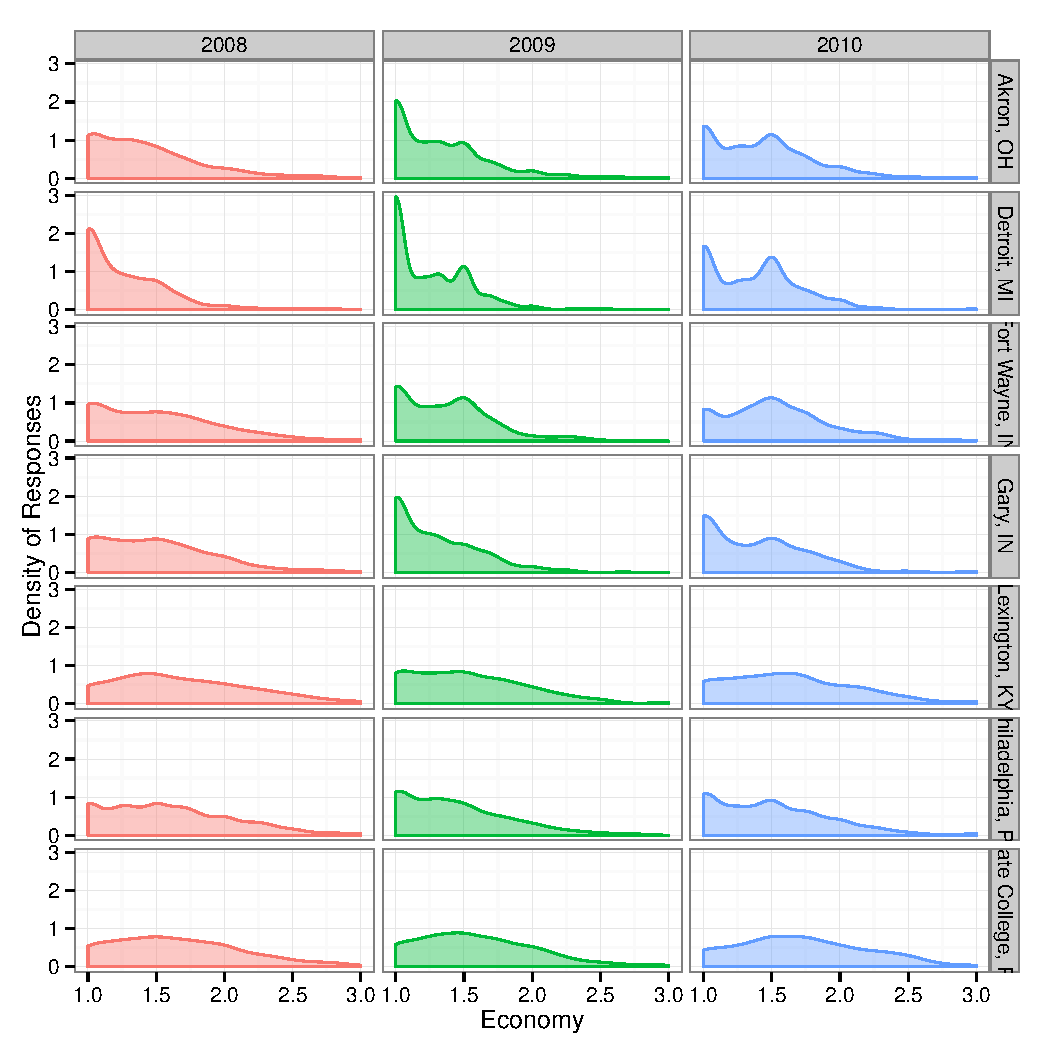
\includegraphics[width=\maxwidth]{figure/rb_one} \caption[Caption]{Caption...\label{fig:rb_one}}
\end{figure}


\end{knitrout}



\section*{Conclusion}

This is the conclusion.


\printbibliography
\end{document}
